\documentclass[11pt]{article}
\usepackage[letterpaper,margin=1in]{geometry}
\usepackage[T1]{fontenc}
\usepackage{mathptmx}
\usepackage{amsmath,amssymb}
\usepackage{graphicx}
\usepackage{booktabs}
\usepackage{threeparttable}
\usepackage[font=small,labelfont=bf]{caption}
\usepackage[numbers,sort&compress]{natbib}
\usepackage{xcolor}
\usepackage{microtype}
\usepackage{authblk}
\usepackage[colorlinks=true,linkcolor=blue!50!black,citecolor=blue!50!black,urlcolor=blue!50!black]{hyperref}
\setlength{\emergencystretch}{3em}
\renewcommand{\baselinestretch}{1.12}
\newcommand{\chitwo}{\chi^{(2)}}
\newcommand{\um}{\,\mu\mathrm{m}}

\title{Electrically written quasi-phase matching of intersubband second-harmonic generation: bias-reversed asymmetric and mirror-symmetric quantum wells}
\author{Gracen Ownby}
\affil{University of Oklahoma, Norman, Oklahoma, USA}
\date{\small 14 October 2026}

\begin{document}
\maketitle

\begin{abstract}
Resonant intersubband nonlinearities in quantum wells exceed those of bulk crystals by orders of magnitude, but in waveguides they are limited by phase mismatch, resonant absorption and saturation. Quasi-phase matching (QPM) written by the bias of segmented electrodes was proposed in the patent literature, but it has not been established whether such a scheme can compete with growth-defined orientation reversal or with Stark on/off QPM. We compare two mechanisms for bias-defined QPM. In an ordinary asymmetric double quantum well (ADQW), bipolar bias Stark-shifts the 1--2 transition to either side of the pump, which reverses the phase of the resonant $\chitwo$ (163--199$^\circ$ between segments) while detuning both segments, so they saturate less. In a mirror-symmetric coupled triple well, the field localizes the ground state in one outer well, so the structure behaves as an ADQW whose orientation follows the field; $\chitwo$ is exactly odd and the linear response exactly even in the field, so alternating polarity writes an exact sign grating. For In$_{0.53}$Ga$_{0.47}$As/In$_{0.52}$Al$_{0.48}$As structures pumped at 10$\um$, self-consistent Schr\"odinger--Poisson calculations with depolarization give the triple well (58/14/34/14/58~\AA) $|\chitwo|=61$~nm/V at 55~kV/cm, 55\% of an optimized ADQW, robust to model, material and linewidth variations; symmetric single, double and stepped wells reach 34--40\% only at 140~kV/cm, the highest field at which our single-period model is valid. In an InP waveguide, segmented electrodes at 30~V retain 92\% of the ideal sign-reversal coefficient. Coupled-wave simulations with LO-phonon-resolved multilevel saturation and pump depletion, with every field restricted to where a single-period model is valid, give the following. The ADQW under bipolar bias ($\pm60$--120~kV/cm) is the most efficient scheme above 1~W, by 1.7--2.2 times over the bias-optimized triple well. The triple well in turn gives 1.6--2.6 times the conversion of Stark on/off QPM at 1.26~W and 1.1--1.6 times at 10~W, and 1.6--9.0 times that of an ADQW with growth-defined orientation reversal at 1.26--20~W. At 10~mW all electrical schemes are within a factor of 1.5 of each other. Absolute efficiencies (0.10--0.89\% at 10~W for the triple well at its design field) depend on the relaxation pathways. Bias-defined phase reversal near resonance therefore does not need mirror symmetry, and the bipolar ADQW is the choice for efficiency; the triple well offers an exact sign grating with identical segments, no absorption or index grating at the QPM period and a bias-independent period. We give a growth- and fabrication-ready triple-well design, its operating constraints, and the measurements that would test it.
\end{abstract}

\section{Introduction}
Intersubband (ISB) transitions in doped semiconductor quantum wells (QWs) can be engineered to place two or three transitions in resonance with a pump and its harmonic, giving second-order susceptibilities $\chitwo$ of order $10^4$--$10^6$~pm/V in the mid-infrared \cite{Fejer1989,Rosencher1991,Rosencher1996,Meyer1995,Vurgaftman1996,Vurgaftman2021}. These nonlinearities underpin difference-frequency terahertz sources integrated into mid-infrared quantum cascade lasers (QCLs) \cite{Belkin2007,Fujita2018} and nonlinear polaritonic metasurfaces \cite{Lee2014,Sarma2020,Yu2022,Yu2024,Krakofsky2023}. In waveguides, however, the resonant enhancement comes with strong absorption at both frequencies, saturation at MW/cm$^2$ intensities \cite{Boucaud1991}, and a coherence length $L_\mathrm{coh}=\pi/\Delta k$ of only tens of micrometres, so the useful interaction length is short and the conversion efficiency is low \cite{Vurgaftman2021,Vurgaftman1996,Chesi2023}.

Several routes to phase matching have been explored in QW structures. True phase matching has been obtained by adding QWs whose resonant dispersion compensates the material and waveguide dispersion \cite{Vurgaftman1996,Vodopyanov1998}, and Meyer \emph{et al.} proposed imposing it electrically through the voltage dependence of that resonant index \cite{Meyer1995APL}; Vurgaftman \emph{et al.} showed that a uniform field across an InGaAs/InAlAs ADQW waveguide moves the resonant contribution to the index mismatch enough to switch a 50-$\mu$m, 14\% converter off at $-25$~kV/cm, or to keep at least 1\% conversion from 9 to 20~$\mu$m pump wavelength; there the field is uniform and acts on the coherence length, not on the sign of $\chitwo$, and they proposed separating the active and phase-matching regions \cite{Vurgaftman1996SSC,VurgaftmanNLO1996}. Quasi-phase matching (QPM) has been implemented by growing asymmetric coupled wells with periodically reversed orientation \cite{Janz1994,Fiore1997}, by spatially selective intermixing that switches $\chitwo$ off in alternate domains \cite{Bouchard2000,Zeaiter2003}, and by periodically Stark-detuning ISB resonances along a QCL ridge \cite{Belkin2006}. Magnitude modulation is weaker than sign reversal: an ideal on/off pattern has a first Fourier coefficient of $1/\pi$ against $2/\pi$ for sign reversal, a factor of four in conversion efficiency. Stark detuning also changes the linear absorption and refractive index from segment to segment. Near resonance, however, a Stark shift that moves a transition across the pump also reverses the phase of $\chitwo$; we show in Secs.~\ref{sec:eff} and \ref{sec:opt} that this route, with bipolar bias on an ordinary ADQW, is the most efficient electrical pattern we have found. Bias control of this detuning phase has been demonstrated in intersubband polaritonic metasurfaces \cite{Yu2025}; here we apply it along a waveguide to quasi-phase-match. Orientation reversal by growth fixes the period at epitaxy and requires regrowth or patterned growth. Outside QWs, field-induced $\chitwo=3\chi^{(3)}E$ is sign-reversed with alternating junctions in silicon \cite{Timurdogan2017} and programmed optically in silicon nitride \cite{Yanagimoto2026}, but the induced nonlinearity is small (0.5--41~pm/V) and needs tens to a thousand volts.

That a perpendicular field induces a $\chitwo$ in a symmetric QW whose sign follows the field was predicted \cite{Tsang1988} and observed \cite{Fejer1989}. A 1989 patent proposed spatially periodic biasing of such wells in a waveguide for QPM \cite{Patent4880297}, and a 1994 patent described $+\chitwo$ and $-\chitwo$ zones written by the direction of the field in a symmetric (stepped) well \cite{Patent5289309}. We are not aware of a quantitative design of this scheme, a comparison with established QPM methods and with other bias patterns, or a demonstration. The obstacle is magnitude: in a symmetric single or stepped well, $\chitwo$ grows only gradually with field and remains well below that of an ADQW. Here we ask whether QPM written by the bias of segmented electrodes can compete with growth-defined orientation reversal and with Stark on/off QPM, and we examine two routes: bipolar bias on an ordinary ADQW, which reverses the phase of the resonant $\chitwo$ by Stark detuning, and a mirror-symmetric coupled triple well, which removes the magnitude obstacle of symmetric wells and writes an exact sign grating. Our contributions are: (i) a comparison of the electrical schemes with growth-defined orientation reversal, Stark on/off QPM and phase matching in a common waveguide, electrode and saturated coupled-wave model with LO-phonon-resolved relaxation, including fully optimized two-field bias patterns, which shows that bias-defined QPM is competitive above about 1~W and that the bipolar ADQW is the most efficient electrical scheme; (ii) the first route, bipolar bias on an ADQW, with the phase reversal by detuning quantified at the optimum fields and its costs (unequal segments, an absorption and index grating at the QPM period) identified; (iii) the second route, a mirror-symmetric triple well that acts as an \emph{electrically reversible} ADQW, reaching about half of an optimized ADQW's $\chitwo$ at 55~kV/cm, whereas symmetric single, double and stepped wells reach 34--40\% only at 140~kV/cm, the highest field at which our model is valid, together with an exact symmetry argument showing that bias reversal writes a pure sign grating, with the residual linear modulation quantified; (iv) a self-consistent analysis, including the electrons' own space charge and depolarization, with an explicit error budget; and (v) a design, its operating constraints and a test plan specific enough to be grown and measured.

\section{Concept}
Let $\Pi$ be the mirror operation $z\to -z$ about the centre of a structure whose layer sequence is symmetric. The Hamiltonian with a uniform field $F$ along $z$ satisfies $\Pi H(F)\Pi^{-1}=H(-F)$. Its eigenstates at $-F$ are therefore the mirror images of those at $+F$, with identical energies and with dipole matrix elements $z_{ij}(-F)=-z_{ij}(F)$ (up to the arbitrary signs of the states, which cancel in closed loops). Every term of the second-order susceptibility contains a closed loop of three dipoles, $z_{lm}z_{mn}z_{nl}$, so
\begin{equation}
\chitwo(-F)=-\chitwo(F),\qquad \chitwo(0)=0, \label{eq:odd}
\end{equation}
while every linear quantity, which contains $|z_{lm}|^2$, is even in $F$. A periodic electrode pattern of alternating polarity therefore produces a pure sign grating of $\chitwo$: oppositely biased segments have identical linear absorption and refractive index (the gaps between electrodes are treated in Sec.~\ref{sec:wg}). The same argument holds when the electrons' own Hartree potential and depolarization are included, provided the doping is placed mirror-symmetrically.

The open question is magnitude. A symmetric single well acquires $\chitwo$ only linearly in $F$ at small fields \cite{Fejer1989}. A coupled triple well (Fig.~\ref{fig:concept}a) behaves differently. Its two outer wells form a near-degenerate pair (splitting 11~meV at zero field), so a modest field localizes the ground state in one outer well, and the structure then resembles an ADQW of outer well, barrier and centre well. The polarity of $F$ selects which outer well, and hence the orientation of the effective ADQW. Fig.~\ref{fig:concept}b shows the device: a waveguide containing a stack of such triple wells, with segmented top electrodes of alternating polarity over a common ground contact.

\begin{figure}[t]
\centering
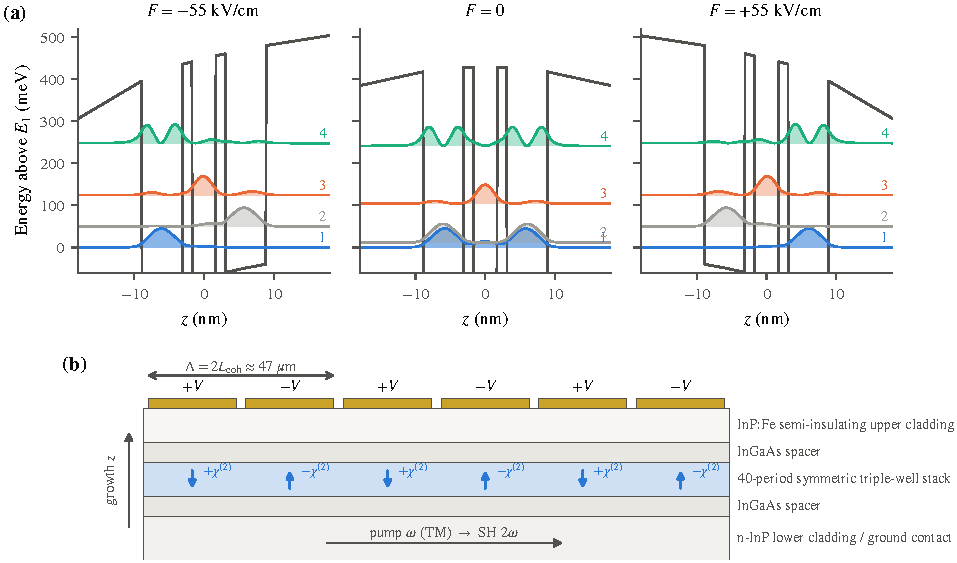
\includegraphics[width=\textwidth]{figures/fig1_concept.pdf}
\caption{(a) Self-consistent conduction-band profile and probability densities of the lowest four subbands of the 58/14/34/14/58~\AA\ InGaAs/InAlAs triple well at $-55$, 0 and $+55$~kV/cm (300~K, $5\times10^{11}$~cm$^{-2}$ per period). At zero field the ground state is shared by the two outer wells and $\chitwo=0$; a field localizes it in one outer well, forming an effective ADQW whose orientation follows the field. (b) Device concept: segmented electrodes of alternating polarity over a grounded n-InP contact reverse the sign of $\chitwo$ every coherence length.}
\label{fig:concept}
\end{figure}

\section{Model}
\subsection{Electronic structure and nonlinear susceptibility}
We use a single conduction band with the BenDaniel--Duke kinetic operator \cite{BenDaniel1966} and Kane-type nonparabolicity, $m^*(z,E)=m^*_0(z)\,[1+(E-V(z))/E_g(z)]$ \cite{Nelson1987}, for In$_{0.53}$Ga$_{0.47}$As wells ($m^*_0=0.043$, $E_g=0.75$~eV) and In$_{0.52}$Al$_{0.48}$As barriers ($m^*_0=0.075$, $E_g=1.45$~eV) with a 0.52~eV conduction-band offset \cite{Vurgaftman2001}. The Schr\"odinger equation is discretized on a cell-centred 0.5~\AA\ grid, which makes mirror-symmetric stacks exactly symmetric on the grid. Each state is found self-consistently with its own energy-dependent mass by requiring that it remain the $k$-th eigenvalue of $H(E)$; this preserves node counting and avoids state swapping. The resulting states are not exactly orthogonal and are L\"owdin-orthonormalized \cite{Lowdin1950} together with the states of the computational box above them, which makes the dipoles independent of the box. Using instead the two-band Kane states, which are orthogonal without the L\"owdin step (overlaps between localized states below $10^{-4}$), changes $|\chitwo|$ at the pump by $-0.9\%$ for the ADQW used below (64/10/29~\AA) and by $-0.7\%$ for the triple well at 55~kV/cm. Only states with at least 80\% of their probability in the active region are kept.

The resonant SHG susceptibility for arbitrary subband populations $\rho_l$ is the density-matrix result \cite{Boyd2008,Rosencher1991}
\begin{equation}
\chitwo(2\omega;\omega,\omega)=\frac{Ne^3}{\varepsilon_0}\sum_{l,m,n}\frac{z_{lm}z_{mn}z_{nl}}{\tilde E_{nl}-2\hslash\omega-i\Gamma}\left[\frac{\rho_l-\rho_m}{\tilde E_{ml}-\hslash\omega-i\Gamma}-\frac{\rho_m-\rho_n}{\tilde E_{nm}-\hslash\omega-i\Gamma}\right],\label{eq:chi}
\end{equation}
where $N$ is the electron density averaged over a period, $\Gamma=10$~meV is the half-width at half-maximum of each transition, and $\tilde E_{ml}$ are depolarization-shifted transition energies (Sec.~\ref{sec:sc}). Eq.~(\ref{eq:chi}) is invariant under a shift of the coordinate origin, contains the permanent-dipole term $z_{12}^2(z_{22}-z_{11})$ automatically, and reduces to the three-level expression of Ref.~\cite{Vurgaftman2021} when only the ground state is occupied. Populations follow Fermi--Dirac statistics at 300~K for a sheet density $n_s$ per period. We compare designs at fixed $n_s=5\times10^{11}$~cm$^{-2}$ per period with a 200~\AA\ In$_{0.52}$Al$_{0.48}$As spacer, so that both structure types hold the same number of electrons per period.

\subsection{Self-consistent electrostatics and depolarization}\label{sec:sc}
Donors are placed as sheets at the centres of the spacers (mirror-symmetric). The stack is voltage-biased, so the period-averaged field equals the applied $F$ and the Hartree field has zero mean over a period. We solve Poisson's equation periodically with position-dependent permittivity (13.9 for InGaAs, 12.4 for InAlAs) and iterate to self-consistency, to $10^{-5}$~eV in the potential. Depolarization shifts follow Ando \emph{et al.} \cite{Ando1982}, applied transition by transition with an average permittivity $\varepsilon=13.5$:
\begin{equation}
\tilde E_{ml}^2=E_{ml}^2\left[1+\frac{2e^2n_s(\rho_l-\rho_m)S_{lm}}{\varepsilon\varepsilon_0E_{ml}}\right],\quad S_{lm}=\int dz\left[\int_{-\infty}^{z}\psi_l\psi_m\,dz'\right]^2 .
\end{equation}
Exciton-like corrections, coupling between transitions, and the local-field correction of the driving field \cite{Zaluzny1995,Heyman1994} are not included.

\subsection{Waveguide, electrodes and propagation}
TM modes of the planar waveguide are computed by finite differences for $H_y$ with complex permittivities. InP follows the Pettit--Turner dispersion \cite{Pettit1965}; InGaAs and InAlAs are taken as $n=3.43$ and $3.20$ at 10$\um$ with the same dispersion as InP; n-InP is described by a Drude term; and gold electrodes use Ordal's Drude parameters \cite{Ordal1985}. The stack's z-polarized response is entirely its ISB response and is treated in the propagation model rather than as free-carrier absorption.

The field under the electrodes is the Fourier-series solution of Laplace's equation between a segmented top plane (segments $\pm V$ separated by gaps with linearly varying potential) and a grounded bottom contact, for a uniform permittivity (the layers differ by less than 12\%). Local $\chitwo(F(x))$ is taken from the self-consistent $\chitwo(F)$ curve, and the QPM coefficient is the first Fourier component $c_1=|\Lambda^{-1}\int_0^\Lambda\chitwo(x)e^{-2\pi ix/\Lambda}dx|$, equal to $(2/\pi)|\chitwo|$ for an ideal sign-reversed square wave.

Propagation uses mode amplitudes $a_{1,2}$ ($|a|^2$ is power) generalizing Eq.~(15.29) of Ref.~\cite{Vurgaftman2021}:
\begin{align}
\frac{da_1}{dx}&=-\frac{\alpha_1}{2}a_1-iK\,s(x)\,\chitwo{}^*\,a_2a_1^*\,e^{-i\Delta k x},\\
\frac{da_2}{dx}&=-\frac{\alpha_2}{2}a_2-iK\,s(x)\,\chitwo\,a_1^2\,e^{+i\Delta k x},\qquad K=\frac{\pi}{\lambda_1}\sqrt{\frac{2\,\mathcal{O}}{n_1^2n_2c\varepsilon_0}},
\end{align}
where $\mathcal{O}=|\int_\mathrm{QW}f_1^2f_2^*\,dz|^2/w$ is the nonlinear overlap of the normalized TM fields $f_{1,2}$ for a ridge of width $w=15\um$, and $s(x)$ is the QPM pattern. The modal losses are $\alpha_j=\Gamma_j\alpha_{\mathrm{ISB},j}(\rho)+\alpha_{\mathrm{bg},j}$. Saturation enters through steady-state rate equations for all subband populations,
\begin{gather}
0=\sum_l W_{lm}(\rho_l-\rho_m)+\sum_l\left[R_{lm}(\rho_l-\rho_l^{(0)})-R_{ml}(\rho_m-\rho_m^{(0)})\right],\label{eq:rate}\\
W_{lm}=\frac{\sigma_{lm}(\omega)I_1}{\hslash\omega}+\frac{\sigma_{lm}(2\omega)I_2}{2\hslash\omega},\nonumber
\end{gather}
with per-electron cross-sections $\sigma_{lm}$ from the depolarization-shifted Lorentzian transitions, local intensities $I_j=P_j\Gamma_j/(t_\mathrm{stack}w)$, and equilibrium (Fermi--Dirac) populations $\rho^{(0)}$. The relaxation rates $R_{lm}$ from subband $l$ to $m$ are computed for each structure from the Fr\"ohlich interaction with bulk LO phonons \cite{Ferreira1989},
\begin{gather}
R_{lm}=\frac{e^2m^*\omega_\mathrm{LO}}{4\varepsilon_0\hslash^2}\left(\frac{1}{\varepsilon_\infty}-\frac{1}{\varepsilon_s}\right)\left[(n_\mathrm{LO}+1)\frac{I(Q_e)}{Q_e}+n_\mathrm{LO}\frac{I(Q_a)}{Q_a}\right],\label{eq:lo}\\
I(Q)=\iint\psi_l(z)\psi_m(z)\,\psi_l(z')\psi_m(z')\,e^{-Q|z-z'|}\,dz\,dz',\nonumber
\end{gather}
for electrons at the bottom of subband $l$ with $E_l>E_m$, where $\hslash^2Q_{e,a}^2/2m^*=E_l-E_m\mp\hslash\omega_\mathrm{LO}$ (emission only if positive) and $n_\mathrm{LO}$ is the 300~K phonon occupation; upward rates follow from detailed balance. We use $\hslash\omega_\mathrm{LO}=33.7$~meV, $\varepsilon_\infty=11.6$, $\varepsilon_s=13.9$ and $m^*=0.043$ for In$_{0.53}$Ga$_{0.47}$As. Interface-roughness, alloy and electron--electron scattering are neglected; we test their effect by adding a 1~ps channel to the ground state, and we repeat the comparison with a single relaxation time $\tau=1$~ps for all transitions \cite{Vurgaftman2021}. Because $\chitwo$ and $\alpha_\mathrm{ISB}$ in Eq.~(\ref{eq:chi}) are linear in $\rho$, both are recomputed exactly at every step. The phase mismatch includes the modal dispersion and each medium's own ISB contribution to the refractive index. For segmented schemes in which the medium changes from segment to segment (Stark on/off QPM), each segment has its own $\chitwo$, absorption, relaxation and phase mismatch, and its length equals its own coherence length.

\subsection{Validation}
All numbers come from the open-source package \texttt{qwkit} (v0.6.1), supplied with this article together with the scripts and data for every figure and table. Its 57 automated tests include those summarized in Table~\ref{tab:validation}. The LO-phonon benchmark agrees to 13\%, within the uncertainty from the unstated $\varepsilon_\infty$ of the reference calculation. The symmetry tests are the most demanding: earlier versions of the solver produced a small spurious $\chitwo$ at zero field, from grid asymmetry, state swapping and non-orthogonality, and the tests were written to catch exactly these errors.

\begin{table}[t]
\centering\small
\caption{Validation tests in \texttt{qwkit} v0.6.1 (all pass).}\label{tab:validation}
\begin{tabular}{@{}ll@{}}
\toprule
Test & Criterion \\ \midrule
Infinite-well limit & energies within 1\%, $z_{12}$ within 2\% of analytic \\
Book Eq.~(15.28) three-level limit & Eq.~(\ref{eq:chi}) within 5\% \\
Symmetric wells (fixed and self-consistent potential) & $\chitwo(0)=0$ and $\chitwo(-F)=-\chitwo(F)$ to $10^{-6}$ relative \\
Translation invariance & $\chitwo$ unchanged by origin shift to $10^{-9}$ \\
State parity with nonparabolicity & exact parity, strictly ordered energies \\
Charged-sheet electrostatics & potential within 1\% of analytic \\
Self-consistency & charge neutrality $<10^{-6}$; convergence $<10^{-5}$~eV \\
Depolarization & blue shift for populated ground state; vanishes as $n_s\to0$ \\
Symmetric dielectric slab, TM$_0$ & $n_\mathrm{eff}$ within $2\times10^{-4}$ of analytic \\
Parallel-plate electrodes & field within 1\% of $V/d$ \\
QPM coefficients & $2/\pi$ (sign reversal) and $1/\pi$ (on/off) within $10^{-3}$ \\
Undepleted, lossless, phase-matched SHG & $P_2=\eta_nP_1^2L^2$ within $10^{-3}$ \\
Lossless depletion & $P_1+P_2$ conserved to $10^{-6}$ \\
Two-level saturation & population difference and absorption halve at $I_\mathrm{sat}$ \\
LO-phonon form factor $I(Q)$ & direct double sum to $10^{-9}$ \\
Form factor, short-range limit & $I(Q)\to(2/Q)\int\psi_l^2\psi_m^2dz$ within 1\% \\
LO-phonon benchmark (10~nm GaAs well \cite{nextnano}) & $E_{21}$ within 0.3~meV; $\tau_{21}=0.73$ vs 0.83~ps \\
Detailed balance & Boltzmann populations stationary to $10^{-6}$ \\
Level-resolved rate equations & equilibrium stationary; populations conserved \\
Segmented propagation & reproduces sign-reversal QPM to $10^{-6}$ \\ \bottomrule
\end{tabular}
\end{table}

\section{Results}
\subsection{Symmetric designs against an optimized ADQW}
We optimized an ADQW (wide well, barrier, narrow well) and four symmetric families (single, double, triple and stepped wells) for a 10$\um$ pump at fixed $n_s$, first with a fixed potential and then self-consistently. The best ADQW is 64/10/29~\AA, with $|\chitwo|=110.9$~nm/V in the full model. Fig.~\ref{fig:chi}a shows the best symmetric designs as a function of field. The triple well rises steeply, reaching 55\% of the ADQW at 55~kV/cm; the best triple well found in the self-consistent search (59/12/36~\AA) reaches 57\% at 65~kV/cm, and we retain 58/14/34~\AA\ for its lower operating field. Up to 140~kV/cm, the highest field at which we consider the single-period model valid (Sec.~\ref{sec:eff}), the symmetric double and single wells reach only 39\% and 40\%, both at that limit. Their $|\chitwo|$ keeps rising at higher fields (to 90\% for the double well at 200~kV/cm), but there their third subband lies above the barrier band edge at the period boundary, where a single-period model no longer describes it. We also optimized the symmetric stepped well of Ref.~\cite{Patent5289309}, an InGaAs core between In$_{0.53}$(Ga$_{1-x}$Al$_x$)$_{0.47}$As steps inside InAlAs barriers, over core width (20--80~\AA), step width (10--60~\AA), step composition ($x=0.2$--0.5, parameters interpolated linearly between the ternaries) and field. The design shown in Fig.~\ref{fig:chi}a, 50/40/50~\AA\ with $x=0.35$, reaches 25\% at 140~kV/cm, and no refined candidate exceeds 34\% up to that field; higher values (up to 48\% at 180~kV/cm) again occur only beyond it.

Fig.~\ref{fig:chi}b shows the mechanism. At zero field the outer-well doublet is split by 11~meV and $z_{13}=0$ by parity. With field, the doublet splits and the ground-state centroid moves to $|\langle z\rangle_1|=5.7$~nm at 55~kV/cm, close to the outer-well centre at 6.0~nm. At 55~kV/cm the ladder $1\to3\to4$ is doubly resonant ($E_{31}=124.4$~meV, $E_{41}=247.8$~meV against $\hslash\omega=124.0$~meV), with $z_{13}=1.24$, $z_{34}=2.40$ and $z_{14}=1.12$~nm.

\begin{figure}[t]
\centering
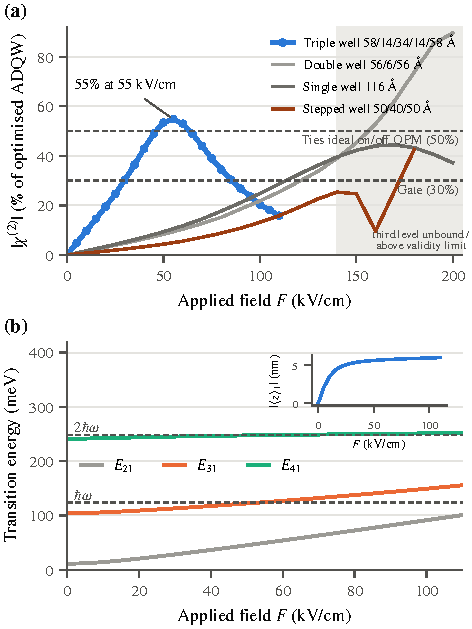
\includegraphics[width=0.52\textwidth]{figures/fig2_chi_vs_field.pdf}
\caption{(a) $|\chitwo|$ of the best symmetric designs as a percentage of the optimized ADQW, versus applied field, full self-consistent model (300~K, $n_s=5\times10^{11}$~cm$^{-2}$, $\Gamma=10$~meV, 10$\um$ pump). The shaded region above 140~kV/cm, where the third level lies above the barrier edge at the period boundary, is beyond the range in which the single-period model is valid (Sec.~\ref{sec:eff}); the stepped well (In$_{0.53}$(Ga$_{0.65}$Al$_{0.35}$)$_{0.47}$As steps) has fewer than three localized levels at 170~kV/cm, where its point is omitted, and is shown up to 180~kV/cm. (b) Transition energies of the triple well versus field, with the pump and SH photon energies; inset, ground-state centroid relative to the structure centre.}
\label{fig:chi}
\end{figure}

\subsection{What the self-consistent physics changes}
Table~\ref{tab:ladder} shows the triple-well-to-ADQW ratio at increasing levels of model and for different donor placements. The electrons in the triple well move by $\sim$5.7~nm under bias, but because each period is voltage-clamped the space charge only redistributes the field inside the period: the optimum field shifts from 50 to 55~kV/cm and the ratio stays between 55\% and 63\%. Over $n_s=10^{10}$--$5\times10^{11}$~cm$^{-2}$ the ratio is 55--61\%.

\begin{table}[t]
\centering\small
\caption{Triple well (58/14/34~\AA) against the ADQW (64/10/29~\AA) at different model levels; each design at its optimum field.}\label{tab:ladder}
\begin{tabular}{@{}lcccc@{}}
\toprule
Model & Triple well (nm/V) & Field (kV/cm) & ADQW (nm/V) & Ratio \\ \midrule
Fixed potential, no depolarization & 61.2 & 50 & 105.7 & 58\% \\
Fixed potential, depolarization & 59.3 & 45 & 93.8 & 63\% \\
Hartree, no depolarization & 60.7 & 55 & 103.2 & 59\% \\
\textbf{Hartree + depolarization (full)} & \textbf{60.8} & \textbf{55} & \textbf{110.9} & \textbf{55\%} \\
Full, donors in all wells & 60.1 & 60 & 105.0 & 57\% \\
Full, donors in the centre well & 58.7 & 70 & 105.0 & 56\% \\ \bottomrule
\end{tabular}
\end{table}

\subsection{Robustness}
Fig.~\ref{fig:err} re-evaluates the ratio with the full model under parameter and growth errors, re-tuning the triple well's field in each case (the field is a free parameter of the device) and keeping the ADQW at zero bias. Band-offset ($\pm0.02$~eV), effective-mass ($\pm5\%$) and linewidth (6--14~meV) variations keep the ratio at 53--62\%; the linewidth changes both structures almost equally. A one-monolayer ($\pm3$~\AA) error in the outer wells is the most damaging for the triple well (36--38\%), because those wells set the doublet on which the mechanism relies. The same errors in the ADQW at fixed bias move the ratio to 74--112\%. A biased ADQW could partly re-tune, so the fair conclusion is that both designs require monolayer control, with the triple well's bias acting as a built-in trim.

\begin{figure}[t]
\centering
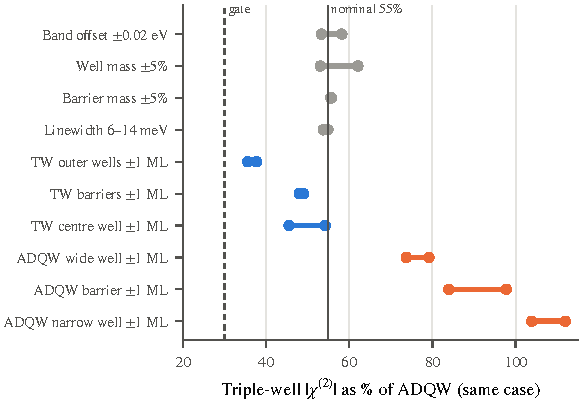
\includegraphics[width=0.52\textwidth]{figures/fig3_error_budget.pdf}
\caption{Error budget: triple-well $|\chitwo|$ as a percentage of the ADQW in the same case (full model). Grey: material parameters and linewidth; blue: triple-well growth errors (field re-tuned); orange: ADQW growth errors (0~V). Dashed line, 30\% design gate; solid line, nominal.}
\label{fig:err}
\end{figure}

\subsection{Waveguide and electrodes}\label{sec:wg}
The waveguide (Fig.~\ref{fig:wg}a) has, from the top, gold electrodes on 2.0$\um$ of semi-insulating InP:Fe, a 0.9$\um$ InGaAs spacer, a 40-period stack (1.51$\um$), a second 0.9$\um$ InGaAs spacer and an n-InP ($10^{17}$~cm$^{-3}$) lower cladding that serves as the ground contact. The TM$_0$ modes have $n_\mathrm{eff}=3.231$ (10$\um$) and 3.338 (5$\um$), confinement factors $\Gamma_1=0.39$ and $\Gamma_2=0.51$, nonlinear overlap $|\int f_1^2f_2^*|^2=0.053\um^{-1}$, and background losses of 3.3 and 0.16~cm$^{-1}$. Because the 5$\um$ mode is much better confined, waveguide dispersion dominates and $L_\mathrm{coh}=23.4\um$ (23.2--25.2$\um$ including each medium's ISB index), much shorter than the 63$\um$ of bulk InP. The electrode period is therefore $\Lambda\approx47\um$.

With the ground plane 5.31$\um$ below the electrodes, 30~V segments give a 56~kV/cm plateau in the stack (Fig.~\ref{fig:wg}b). The field rounds over a few micrometres at segment boundaries, but because $\chitwo(F)$ saturates near its optimum the $\chitwo$ profile stays close to a square wave: the QPM coefficient is 92\% of the ideal $(2/\pi)|\chitwo|_{\max}$ for 2$\um$ gaps (91--93\% for 1--4$\um$).

Because the linear response is even in $F$, the absorption and refractive index are the same under both electrodes and change only where the field passes through zero in the gaps, twice per period. Their modulation therefore has no Fourier component at the QPM wavevector $K=2\pi/\Lambda$; its component at $2K$ is 27~cm$^{-1}$ in the modal pump absorption and $3.1\times10^{-3}$ in the modal pump index, for a plateau modal absorption of 238~cm$^{-1}$. For comparison, Stark on/off switching of the ADQW between 0 and $-80$~kV/cm (the best off field at 10~W, Sec.~\ref{sec:eff}) writes a modal pump-absorption grating of 239~cm$^{-1}$ and an index grating of $5.4\times10^{-3}$ at $K$ itself, and its on and off segments have different coherence lengths (25.2 and 28.9$\um$ at $n_s=5\times10^{11}$~cm$^{-2}$).

\begin{figure}[t]
\centering
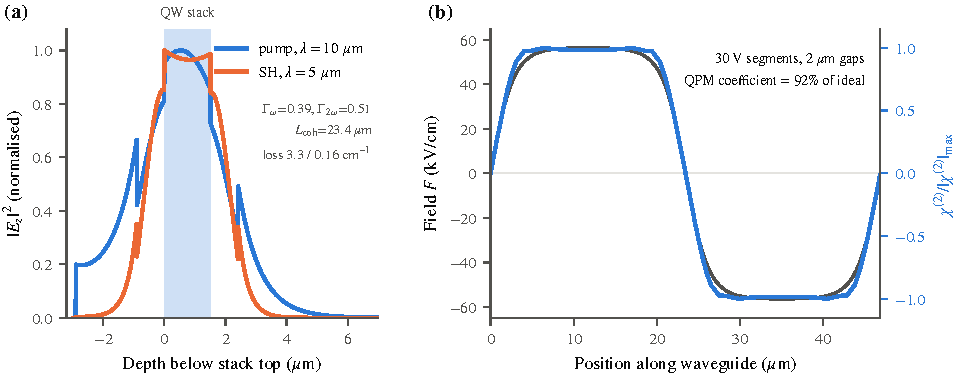
\includegraphics[width=\textwidth]{figures/fig4_waveguide_electrodes.pdf}
\caption{(a) $|E_z|^2$ of the TM$_0$ pump (10$\um$) and SH (5$\um$) modes; the shaded band is the QW stack. (b) Field at mid-stack along one electrode period and the resulting normalized $\chitwo(x)$ for 30~V segments with 2$\um$ gaps.}
\label{fig:wg}
\end{figure}

\subsection{Relaxation and saturation}
The LO-phonon rates of Eq.~(\ref{eq:lo}) give the ADQW's pump level a lifetime of 1.0~ps ($2\to1$) and its SH level 0.53~ps, close to the common 1~ps assumption. The triple well relaxes differently. Its third subband, the upper level of the pump transition, empties mainly into the second subband (0.78~ps), which is localized in the opposite outer well and returns to the ground state in 2.6~ps; at 55~kV/cm the second subband lies 50~meV above the ground state and already holds 17\% of the electrons at equilibrium. Pumping therefore accumulates electrons in the second subband. Even so, the triple well's weaker pump transition (cross-section 2.53 times smaller than the ADQW's $1\to2$) makes it saturate at higher intensity: the small-signal pump absorption halves at 4.0~MW/cm$^2$ in the triple well and 2.0~MW/cm$^2$ in the ADQW (4.8 and 1.7~MW/cm$^2$ with a single 1~ps time), and the triple well's $|\chitwo|$ exceeds the ADQW's above a local pump intensity of 0.9--1.0~MW/cm$^2$ at all doping levels. In the waveguide the intensity in the stack is 1.74~MW/cm$^2$ per watt of pump power.

\subsection{Conversion efficiency with saturation}\label{sec:eff}
Fig.~\ref{fig:prop} and Table~\ref{tab:eff} compare the electrically patterned schemes with growth-defined and idealized benchmarks, all with LO-phonon relaxation and a resonant 10$\um$ pump. Each value is the peak SH power along a waveguide of up to 5~mm, divided by the input pump power.

\paragraph{Triple well.} Sign reversal is evaluated both at the design field of 55~kV/cm, where $|\chitwo|$ is largest, and with the bias amplitude optimized at each doping and power. Both include the 92\% electrode factor.

\paragraph{ADQW configurations.}
\begin{itemize}
\item \emph{Bipolar}: segments at $+F$ and $-F$, with $F$ optimized at each doping and power and the same electrode factor.
\item \emph{Stark on/off}: on at 0~V; off at the field, of either polarity, that maximizes the efficiency. Each segment has its own absorption, index and relaxation.
\item \emph{Idealized on/off}: a pattern that keeps the on-state absorption and index throughout.
\item \emph{Growth reversal}: ideal growth-defined orientation reversal, a lossless $\pm\chitwo$ square wave at 0~V.
\item \emph{No QPM}, and \emph{perfect phase matching}, an unattainable bound.
\end{itemize}

\paragraph{Validity of the fields.} All fields are restricted to $|F|\le140$~kV/cm and to fields where no subband below $E_1+0.40$~eV is only partly localized in the active region. Beyond that, an upper subband anticrosses with states of the field-tilted spacer, which in a real stack belong to the neighbouring periods; a single-period model cannot describe these hybrids, and discarding them misplaces the $2\omega$ resonance. An earlier version of this comparison took the Stark off field as the lowest field at which $|\chitwo|$ fell below 10\% of its 0~V value. For a detuned pump that field was $+170$ to $+230$~kV/cm, where this happens, and the triple well was held at 55~kV/cm. Both choices biased the comparison.

\paragraph{Low pump power.} At 10~mW the ADQW's larger small-signal $\chitwo$ makes growth reversal more efficient than the triple well, and all electrical schemes lie within a factor of 1.5 of each other: the bias-optimized triple well reaches 0.82--1.05 times the bipolar ADQW, 0.74--1.02 times Stark QPM and 0.74--0.99 times growth reversal.

\paragraph{High pump power.} As the power rises, saturation decides:
\begin{itemize}
\item With its bias optimized, the triple well gives 1.6--2.6 times Stark QPM at 1.26~W and 1.06--1.6 times at 10~W. It also gives 1.6--9.0 times the growth-reversed ADQW at 1.26--20~W. At its design field of 55~kV/cm, the triple well is 2.7--4.1 times less efficient at 10~W than with its bias optimized, because its doubly resonant ladder saturates most there.
\item The bipolar ADQW is the most efficient scheme at every doping above 1~W: 1.7--2.2 times the bias-optimized triple well, reaching 2.1\% at 10~W for $n_s=5\times10^{11}$~cm$^{-2}$, above the perfectly phase-matched ADQW (0.31\%).
\end{itemize}

\paragraph{Why the bipolar ADQW wins.} Near resonance the sign of $\chitwo$ follows the sign of the pump detuning. A field of $\pm60$--120~kV/cm Stark-shifts the 1--2 transition of the ADQW to either side of the pump, while the 1--3 transition stays within 16~meV of $2\hslash\omega$. The two segments therefore have $\chitwo$ of nearly opposite phase: the phase difference is 163--199$^\circ$ at the optimum fields, with magnitudes of 15--51\% of the 0~V value. Both segments are detuned, so they absorb and saturate less, the same effect that favours a detuned pump \cite{OwnbyNL02}. Mirror symmetry is therefore not needed for bias-defined phase reversal near resonance. What the triple well adds is an exact sign grating with identical segments.

The Stark on/off scheme also benefits from detuning: its best off segments are detuned rather than switched off. At $n_s=5\times10^{11}$~cm$^{-2}$ they lie at 20--100~kV/cm, and at $-80$~kV/cm the modal pump absorption falls from 838 to 88~cm$^{-1}$ while $|\chitwo|$ keeps 31\% of its 0~V value. It is weaker than the bipolar pattern because one of its segments stays resonant.

\paragraph{Sensitivity to the model.} Table~\ref{tab:sens} tests the comparison at the design field against the model choices that matter most for saturation: linewidths of 6--14~meV, an additional 1~ps relaxation channel, and a single 1~ps relaxation time. The triple well's advantage at 1.26 and 10~W stays between 1.29 and 2.6 over growth reversal. Its ratio to Stark QPM stays between 1.27 and 2.33 at 1.26~W, and between 0.34 and 1.05 at 10~W; the Stark off field is held at its baseline optimum for these variations. The absolute efficiencies are much less robust: at 10~W they range from 0.10 to 0.89\%, because they depend on how fast electrons return to the ground state. The ratios, not the absolute efficiencies, are the predictions of this work.

\paragraph{Detuned pumping.} The comparison above uses a resonant 10~$\mu$m pump. At 10~W the resonant operating point lies beyond the conservative rate-equation limit (Rabi energy equal to the detuned linewidth $|D|$), which for these structures is near 4~W. A companion analysis of saturation limits \cite{OwnbyNL02} shows that a pump tuned 25--35~meV below resonance gives several times higher efficiency inside that limit. We therefore repeat the comparison with the pump red-detuned by up to 40~meV, at $n_s=10^{11}$ and $5\times10^{11}$~cm$^{-2}$. At each wavelength:
\begin{itemize}
\item the waveguide modes, confinement, overlap and background loss are recomputed;
\item each medium's coherence length includes its own ISB index at $\omega$ and $2\omega$;
\item the Stark off field is re-optimized among the valid fields at each photon energy.
\end{itemize}
Table~\ref{tab:detuned} lists each scheme at its own best detuning. The resonant column of Table~\ref{tab:eff} is reproduced to within 2\%. Detuning raises the efficiency of the triple well (by 1.6--4.8 times at its design field), of growth reversal and of phase matching. It also moves most optima to $|D|\gtrsim2\gamma$, where the rate-equation limit (which scales as $|D|^2$) lies at 14--59~W; the optima at $-10$~meV have limits of 8--10~W.

With each scheme at its own best detuning:
\begin{itemize}
\item at 10~W the triple well gives 1.6--1.7 times the growth-reversed ADQW and 1.1--1.6 times Stark QPM;
\item at 4~W it gives 1.07--1.24 and 1.7--2.7 times;
\item at 1.26~W it is comparable to the growth-reversed ADQW (0.86--1.07 times) and gives 1.9--2.2 times Stark QPM.
\end{itemize}
The best Stark points stay closer to resonance ($0$ to $-20$~meV), because the off field already provides the detuning.

\subsection{Optimized bias patterns}\label{sec:opt}
Table~\ref{tab:eff} restricts the bipolar ADQW to symmetric $\pm F$. To test whether either structure gains from more freedom, we also scan general two-field patterns $(F_1,F_2)$, every valid pair from $F\in\{0,\pm20,\dots,\pm120\}$~kV/cm, with the pump detuning scanned from 0 to $-30$~meV and the electrode factor applied to both structures. Table~\ref{tab:opt} lists the optima.

\paragraph{Triple well.} Its best pattern is always symmetric, $\pm F$ with $F=40$--80~kV/cm. Pure sign reversal is the best it can do.

\paragraph{ADQW.} Its optimum is a broad plateau of opposite-polarity patterns at a resonant pump. The symmetric $\pm80$~kV/cm pattern is within 1--8\% of the best pair, $(-80,+120)$, $(-100,+120)$ or $(+120,-120)$~kV/cm, and the patterns are 1.4 times the best triple-well efficiency at 1.26~W and 1.7--2.0 times at 10~W.

\paragraph{Mechanism and prior art.} The mechanism is the phase reversal by detuning described above. The 1--2 resonance is moved by 29--40~meV to either side of the pump, while the 1--3 resonance stays within 13~meV of $2\hslash\omega$, so the harmonic resonance survives; a red-detuned pump instead detunes $2\omega$ by twice as much. Reference~\cite{Vurgaftman1996SSC} used a uniform field on red-detuned transitions to control the resonant index mismatch, and Ref.~\cite{Belkin2006} used Stark detuning to switch $\chitwo$ on and off in alternate segments; neither alternates the polarity from segment to segment to reverse the phase of $\chitwo$. The same detuning phase has been demonstrated directly in ISB polaritonic metasurfaces: in a coupled triple well with equal Stark coefficients for $E_{21}$ and $E_{32}$ the complex $\chitwo$ traces a cardioid as the bias is swept, and two meta-atoms with opposite field overlaps per unit cell give independent 0--$2\pi$ phase and on/off amplitude control with two biases, used for electrically programmed second-harmonic phase and amplitude gratings \cite{Yu2025}. That is local phase control in a 500-nm film, with the $\pi$ offset supplied by the resonator geometry; here the detuning phase is used along a waveguide to quasi-phase-match.

\paragraph{Costs.} Its costs relative to the triple well are:
\begin{itemize}
\item unequal segment magnitudes;
\item segments with different coherence lengths (20.1 and 27.7--28.0$\um$ at $n_s=5\times10^{11}$~cm$^{-2}$);
\item an absorption and index grating at the QPM period.
\end{itemize}
Its best patterns also need higher fields, 80--120~kV/cm against 40--80~kV/cm for the triple well.

\begin{table}[t]
\centering\small
\caption{Best periodic two-field bias patterns $(F_1,F_2)$ in kV/cm, with both fields free among valid fields of up to $\pm120$~kV/cm and the pump detuning (meV) scanned from 0 to $-30$~meV; peak conversion efficiency (\%) with LO-phonon relaxation and the 92\% electrode factor applied to both structures.}\label{tab:opt}
\setlength{\tabcolsep}{4pt}
\begin{tabular}{@{}cccccc@{}}
\toprule
$n_s$ (cm$^{-2}$) & Pump & ADQW: $(F_1,F_2)$, detuning & ADQW (\%) & TW: $(F_1,F_2)$, detuning & TW (\%) \\ \midrule
$10^{11}$ & 1.26 W & $(-80,+120)$, 0 & 0.281 & $(\pm60)$, $-10$ & 0.196 \\
$10^{11}$ & 10 W & $(-80,+120)$, 0 & 1.689 & $(\pm70)$, $-10$ & 0.850 \\
$5\times10^{11}$ & 1.26 W & $(-100,+120)$, 0 & 0.353 & $(\pm40)$, $-20$ & 0.260 \\
$5\times10^{11}$ & 10 W & $(+120,-120)$, 0 & 2.143 & $(\pm80)$, $-10$ & 1.260 \\ \bottomrule
\end{tabular}
\end{table}
The triple well's optimum detuning ($-10$ to $-25$~meV) is smaller than that of growth reversal and phase matching ($-25$ to $-35$~meV), and its efficiency falls steeply beyond $-30$~meV. Table~\ref{tab:detuned} holds the triple well at 55~kV/cm.

\begin{table}[t]
\centering\small
\caption{Peak conversion efficiency (\%) with LO-phonon relaxation for each scheme at its own best red detuning of the pump (in meV, in parentheses; scanned 0 to $-40$~meV, Stark to $-35$~meV, with the waveguide recomputed at each wavelength; Stark off field optimized among valid fields at each detuning), and the ratios of the triple well to Stark QPM and to ideal growth reversal.}\label{tab:detuned}
\setlength{\tabcolsep}{3.2pt}
\begin{tabular}{@{}cccccccc@{}}
\toprule
$n_s$ (cm$^{-2}$) & Pump & TW sign & Stark & rev. & PM & TW/Stark & TW/rev. \\ \midrule
$10^{11}$ & 1.26 W & 0.190 ($-10$) & 0.100 ($-10$) & 0.177 ($-25$) & 0.433 ($-25$) & 1.90 & 1.07 \\
$10^{11}$ & 4 W & 0.392 ($-20$) & 0.231 ($-10$) & 0.316 ($-30$) & 0.768 ($-30$) & 1.70 & 1.24 \\
$10^{11}$ & 10 W & 0.667 ($-20$) & 0.584 ($0$) & 0.393 ($-30$) & 0.950 ($-30$) & 1.14 & 1.70 \\
$5\times10^{11}$ & 1.26 W & 0.251 ($-20$) & 0.112 ($-20$) & 0.293 ($-30$) & 0.704 ($-30$) & 2.25 & 0.86 \\
$5\times10^{11}$ & 4 W & 0.636 ($-25$) & 0.238 ($0$) & 0.594 ($-35$) & 1.407 ($-35$) & 2.68 & 1.07 \\
$5\times10^{11}$ & 10 W & 1.213 ($-25$) & 0.757 ($0$) & 0.762 ($-35$) & 1.785 ($-35$) & 1.60 & 1.59 \\ \bottomrule
\end{tabular}
\end{table}

\begin{figure}[t]
\centering
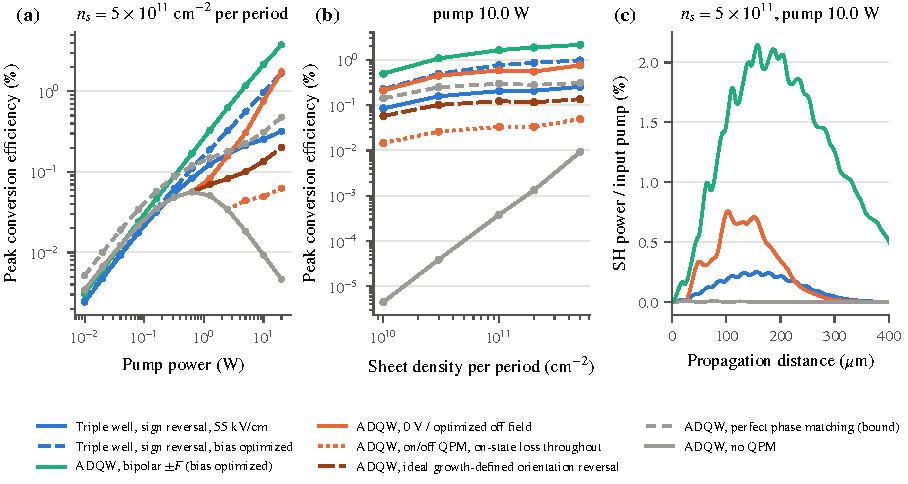
\includegraphics[width=\textwidth]{figures/fig5_propagation.pdf}
\caption{Saturated, pump-depleted SHG in the waveguide of Fig.~\ref{fig:wg}, with LO-phonon relaxation and a resonant pump. (a) Peak conversion efficiency versus pump power at $n_s=5\times10^{11}$~cm$^{-2}$ per period. (b) Peak efficiency versus doping at 10~W. (c) SH power along the waveguide at 10~W and $n_s=5\times10^{11}$~cm$^{-2}$. Schemes: the triple well at 55~kV/cm and with its bias optimized at each point; the ADQW with bipolar segments $\pm F$ ($F$ optimized at each point); Stark modulation between 0~V and the best off field at each point (the off segment is detuned, not switched off); idealized on/off; ideal growth reversal; perfect phase matching; and no QPM. All fields are restricted to those where the single-period model is valid.}
\label{fig:prop}
\end{figure}

\begin{table}[t]
\centering\small
\caption{Peak conversion efficiency (\%) with LO-phonon relaxation, and the corresponding length, for the triple well with sign reversal at 55~kV/cm (TW 55) and with the bias amplitude optimized (TW opt.), and the ADQW with bipolar segments $\pm F$ ($F$ optimized; ADQW bip.), Stark on/off QPM (0~V and the best off field), idealized on/off QPM with on-state loss throughout, ideal growth-defined orientation reversal (rev.), no QPM, or perfect phase matching (PM). Fields are restricted to those where the single-period model is valid; the TW length refers to TW 55.}\label{tab:eff}
\setlength{\tabcolsep}{2.4pt}\footnotesize
\begin{tabular}{@{}ccccccccccc@{}}
\toprule
Pump & $n_s$ (cm$^{-2}$) & TW 55 & TW opt. & ADQW bip. & Stark & on/off (ideal.) & rev. & no QPM & PM & TW length \\ \midrule
1.26 W & $10^{10}$ & 0.065 & 0.075 & 0.128 & 0.046 & 0.012 & 0.046 & $<10^{-4}$ & 0.114 & 2.13 mm \\
1.26 W & $10^{11}$ & 0.115 & 0.164 & 0.279 & 0.067 & 0.019 & 0.063 & 0.003 & 0.153 & 0.30 mm \\
1.26 W & $5\times10^{11}$ & 0.125 & 0.190 & 0.330 & 0.083 & 0.051 & 0.070 & 0.051 & 0.148 & 63 $\mu$m \\
10.0 W & $10^{10}$ & 0.085 & 0.225 & 0.495 & 0.212 & 0.015 & 0.058 & $<10^{-4}$ & 0.142 & 3.95 mm \\
10.0 W & $10^{11}$ & 0.204 & 0.762 & 1.641 & 0.585 & 0.033 & 0.122 & $4\times10^{-4}$ & 0.298 & 0.72 mm \\
10.0 W & $5\times10^{11}$ & 0.254 & 0.972 & 2.147 & 0.759 & 0.049 & 0.135 & 0.009 & 0.311 & 156 $\mu$m \\ \bottomrule
\end{tabular}
\end{table}

\begin{table}[t]
\centering\small
\caption{Sensitivity of the comparison to the linewidth $\Gamma$ (HWHM) and the relaxation model: ratio of the triple well's peak efficiency to the growth-reversed ADQW (TW/rev.) and to Stark QPM (TW/Stark; off field fixed at its baseline optimum). Ranges are over $\Gamma=6$, 10 and 14~meV with LO-phonon relaxation, and over LO-phonon relaxation plus a 1~ps channel and a single 1~ps time at $\Gamma=10$~meV.}\label{tab:sens}
\begin{tabular}{@{}lcccc@{}}
\toprule
$n_s$ (cm$^{-2}$) & Pump & TW/rev. & TW/Stark & TW efficiency (\%) \\ \midrule
$10^{11}$ & 10 mW & 0.87--1.00 & 0.97--1.03 & 0.001--0.007 \\
$10^{11}$ & 1.26 W & 1.29--2.33 & 1.29--2.33 & 0.06--0.34 \\
$10^{11}$ & 10 W & 1.29--1.77 & 0.34--1.05 & 0.10--0.68 \\
$5\times10^{11}$ & 10 mW & 0.70--0.75 & 0.70--0.75 & 0.001--0.008 \\
$5\times10^{11}$ & 1.26 W & 1.33--2.56 & 1.27--2.30 & 0.06--0.39 \\
$5\times10^{11}$ & 10 W & 1.39--2.48 & 0.34--0.86 & 0.12--0.89 \\ \bottomrule
\end{tabular}
\end{table}

\section{Discussion}
\paragraph{Relation to earlier proposals.} Bias-defined sign reversal of a field-induced ISB $\chitwo$ is an old idea \cite{Patent4880297,Patent5289309}; what has been missing is a symmetric structure in which it is large. Up to 140~kV/cm, single, double and stepped symmetric wells give at most 34--40\% of an optimized ADQW, and only at that field, close to the field at which their upper subbands unbind and tunnelling becomes significant. The coupled triple well reaches 55\% at 55~kV/cm because its outer-well doublet converts a modest field into a full localization of the ground state, so that the structure becomes an ADQW of either orientation rather than a weakly perturbed symmetric well. The approach differs from voltage-controlled true phase matching \cite{Meyer1995APL}, which tunes the resonant refractive index and keeps the sign of $\chitwo$ fixed, and from Stark on/off QPM \cite{Belkin2006}, which modulates the magnitude and the linear response together. Bipolar Stark detuning of an ordinary ADQW, which reverses the phase of the resonant $\chitwo$ without mirror symmetry (Sec.~\ref{sec:opt}), is related to the field-modulated detuned resonances of Ref.~\cite{Vurgaftman1996SSC} and is the more efficient electrical pattern in our calculations.

\paragraph{Where the scheme is useful.} Pure sign reversal by bias polarity beats growth-defined orientation reversal where saturation limits conversion, at pump intensities above 0.03--0.5~MW/cm$^2$ in the stack, depending on doping. It is not the most efficient electrical pattern, however. An ordinary ADQW under bipolar bias also reverses the phase of $\chitwo$, by moving its resonance across the pump, and its detuned segments saturate less, so it converts about twice as much at watt-level pumping. The triple well is the better choice when an exact, symmetric sign grating matters: identical segments with one coherence length and loss, no linear grating at the QPM period, and a period that does not depend on the operating point. These properties matter for broadband or tunable operation and for reconfigurable patterns. Because both electrode polarities produce the same linear response, every segment has the same coherence length and loss, so the electrode period and duty cycle do not depend on the bias, doping or pump power; in Stark on/off QPM the on and off segments differ in coherence length by up to 33\% (40\% for the optimized two-field ADQW patterns), and the pattern must be designed for one operating point. Because the period is set by lithography rather than growth, one wafer can carry many periods, and the QPM condition can be trimmed by temperature or by the bias amplitude, which tunes the ISB index.

\paragraph{Practical constraints.} The stack needs about 30~V across 5.3$\um$ with the semi-insulating cladding used here at the 55~kV/cm design field. The bias-optimized patterns of Table~\ref{tab:eff} need 60--90~kV/cm, about 32--48~V; these fields approach the range above about 100--140~kV/cm where upper subbands hybridize with those of neighbouring periods, which a single-period model does not capture. Placing doped contact layers adjacent to the stack would reduce this to about 8~V at the cost of free-carrier loss. Thermionic escape over the 0.40~eV barrier gives an inter-period hopping time of about 0.4~$\mu$s at 300~K (a leakage of $\sim$0.2~A/cm$^2$). Because the semi-insulating cladding blocks this current, the escaping charge accumulates at the stack boundary and would screen a dc bias in roughly the same time. The bias should therefore be pulsed in step with the pump on sub-microsecond time scales, or the device cooled below about 200~K, where the hopping time exceeds a millisecond. Tunnelling escape of the resonant subbands is negligible at 55~kV/cm. The watt-level results imply strong heating: at 10~W and $n_s=5\times10^{11}$~cm$^{-2}$ the stack absorbs 6.9~W over the 156$\um$ optimum length, $1.9\times10^{9}$~W/cm$^3$, an adiabatic heating rate of about 1.3~K/ns. They therefore apply to pulses of about 10~ns or shorter at low duty cycle, or to correspondingly lower powers; continuous-wave operation would require a thermal design not attempted here. The steady-state rate equations are valid for such pulses, which are much longer than the picosecond relaxation times. The outer-well width must be controlled to about a monolayer, which is within current molecular-beam and metal-organic epitaxy practice for QCLs.

\paragraph{Limitations of the model.} We use a single-band model with literature parameters; Lorentzian broadening, which overestimates absorption far from resonance \cite{Vurgaftman2021}; first-order depolarization without excitonic or local-field corrections \cite{Zaluzny1995,Heyman1994}; LO-phonon relaxation for electrons at the subband minima with bulk phonons, without interface-roughness or electron--electron scattering; a planar waveguide and a uniform-permittivity electrode model; linearly interpolated quaternary parameters for the stepped well; and assumed mid-infrared indices for the ternary alloys. These affect the triple well and the ADQW similarly, so the ratios we report are more robust than the absolute values, as the error budget and Table~\ref{tab:sens} confirm. The coherence length depends on the alloy dispersion and must be calibrated experimentally; this is why lithographic periods are attractive.

\paragraph{Extensions.} The same symmetry argument applies to difference-frequency generation of terahertz radiation \cite{Belkin2007,Fujita2018}, provided the nonlinear section is separate from a lasing QCL core, whose bias polarity cannot alternate. It also applies to other material systems with symmetric coupled wells, and to electrically patterned nonlinear metasurfaces \cite{Yu2024,Yu2025}, where bias-programmed phase gratings have now been demonstrated \cite{Yu2025}.

\paragraph{Proposed experiment.} A first test needs one 40-period InGaAs/InAlAs stack on n-InP with the layer sequence of Table~\ref{tab:design}. Three measurements would test the central predictions: (1) ISB absorption at $\pm F$, which should be identical; (2) SHG of a pulsed 10$\um$ pump through a uniform-bias section versus $F$, with bias pulses synchronized to the pump, which should be odd in $F$ and peak near 55~kV/cm; and (3) SHG through segmented sections with a range of electrode periods around 47$\um$, which should show a QPM resonance absent in sections without segmentation.

\begin{table}[t]
\centering\small
\caption{Proposed layer sequence (one period; 40 periods), grown on n-InP.}\label{tab:design}
\begin{tabular}{@{}lll@{}}
\toprule
Layer & Thickness & Notes \\ \midrule
In$_{0.52}$Al$_{0.48}$As spacer & 100 \AA & Si $\delta$-sheet $2.5\times10^{11}$~cm$^{-2}$ at its outer edge \\
In$_{0.53}$Ga$_{0.47}$As outer well & 58 \AA & \\
In$_{0.52}$Al$_{0.48}$As barrier & 14 \AA & \\
In$_{0.53}$Ga$_{0.47}$As centre well & 34 \AA & \\
In$_{0.52}$Al$_{0.48}$As barrier & 14 \AA & \\
In$_{0.53}$Ga$_{0.47}$As outer well & 58 \AA & \\
In$_{0.52}$Al$_{0.48}$As spacer & 100 \AA & Si $\delta$-sheet $2.5\times10^{11}$~cm$^{-2}$ at its outer edge \\ \bottomrule
\end{tabular}
\end{table}

\section{Conclusion}
Quasi-phase matching of intersubband second-harmonic generation can be written electrically, by segmented electrodes of alternating polarity, and it competes with growth-defined orientation reversal and Stark on/off QPM once saturation limits the conversion. We analysed two routes with self-consistent electrostatics, depolarization, growth errors, a realistic waveguide and electrode geometry, and LO-phonon-resolved saturable propagation.
\begin{itemize}
\item An ordinary ADQW under bipolar bias is the most efficient electrical scheme, about twice as efficient as the bias-optimized triple well above 1~W, because a Stark shift across the pump reverses the phase of its resonant $\chitwo$ and detunes both segments. This applies the detuning-phase control demonstrated in intersubband metasurfaces \cite{Yu2025} along a waveguide.
\item A mirror-symmetric coupled triple well is an electrically reversible asymmetric quantum well that retains about half of an optimized ADQW's nonlinearity at 55~kV/cm. Its $\chitwo$ is exactly odd in the field and its linear response exactly even, so alternating-polarity electrodes write an exact sign grating with identical segments, no linear grating at the QPM period and a bias-independent period.
\item With its bias optimized, the triple well outperforms growth-defined orientation reversal by 1.6--9.0 times above about 1~W and Stark on/off QPM by up to 2.6 times near 1~W.
\end{itemize}
Bias-defined phase reversal near resonance therefore does not require mirror symmetry. The bipolar ADQW is the choice for efficiency; the triple well is the choice where an exact, symmetric sign grating matters, and it gives a long-standing proposal for bias-defined QPM a concrete design. Both can be grown and tested with standard InP-based QCL technology, with pulsed bias and pump.

\bibliographystyle{unsrtnat}
\bibliography{refs}

\end{document}
